\chapter[Fake-tau estimation]{Fake-$\hadtau$ estimation}
\label{app:ch8_fake_tau}

The fake-$\hadtau$ background from $\znunu$+jets is estimated using the strategy described in Section~\ref{sec:ch8_strategy}.
Its modelling is tested in a $\zll$ validation region (ZVR).

The ZVR requires two signal electrons or two signal muons and exactly one $\hadtau$ candidate, with the dilepton mass restricted to the $Z$-boson mass window.
A $b$-jet veto and looser selections than in the SRs are applied to increase the event yield, and both lepton channels are used.
The quantity $|\vec p_{\mathrm{T}}^{\,\ell\ell}+\mpt|$ is used to emulate the $\met$ in $\znunu$ events by adding the dilepton momentum to $\mpt$.
An additional requirement of $\pT^{\ell\ell}>130~\GeV$ suppresses the $\ttbar$ background and increases the $\zjets$ purity.
The definition is summarised in Table~\ref{tab:app_ch8_zvr_selections}.

\begin{table}[htbp]
    \centering
    \small
    \caption[Event selections for the ZVR]{Event selection criteria for the ZVR.}
    \label{tab:app_ch8_zvr_selections}
    \begin{tabular}{lcc}
        \toprule
         & \textbf{ZVR selections} & \\
         & \multicolumn{2}{c}{Criterion} \\
        Feature & Muon channel & Electron channel \\
        \midrule
        Trigger & Lowest-unprescaled $\met$ trigger & Single-electron trigger \\
        Lepton multiplicity & $N_\mu=2$ & $N_e=2$ \\
        $\hadtau$ multiplicity & \multicolumn{2}{c}{$N_{\hadtau}=1$} \\
        $b$-jet multiplicity & \multicolumn{2}{c}{$N_b=0$} \\
        Jet multiplicity & \multicolumn{2}{c}{$N_j\geq1$} \\
        Multijet suppression & \multicolumn{2}{c}{$\minDphiJetMet>0.4\quad\text{or}\quad\metOverMinDphiJetPt>6$} \\
        \midrule
        $\pT^{\hadtau}$ & \multicolumn{2}{c}{$>100~\GeV$} \\
        $\mT(\pT^\ell,\met)$ & \multicolumn{2}{c}{$>100~\GeV$} \\
        $m_{\ell\ell}$ & \multicolumn{2}{c}{$[75,105]~\GeV$} \\
        $|\vec p_{\mathrm{T}}^{\,\ell\ell}+\mpt|$ & \multicolumn{2}{c}{$>200~\GeV$} \\
        $\pT^{\ell\ell}$ & \multicolumn{2}{c}{$>130~\GeV$} \\
        $N_j$ & \multicolumn{2}{c}{$\leq3$} \\
        \bottomrule
    \end{tabular}
\end{table}

A total of 116 data events are selected in the ZVR, with a simulated $\zjets$ purity of approximately $90\%$.
The $\pT^{\hadtau}$ and RNN-score distributions are shown in Figures~\ref{fig:ch8_zvr_pt} and~\ref{fig:ch8_zvr_rnn}, respectively.
The simulation overestimates the data by about $50\%$ at high $\pT^{\hadtau}$.
Both the fake-$\hadtau$ rate and the $\zjets$ kinematics can contribute to this disagreement.
However, agreement between data and simulation is observed at low RNN scores, in the $\hadtau$-veto region.
The discrepancy is therefore attributed mainly to the modelling of the fake-$\hadtau$ rate.

This study motivates the conservative normalisation uncertainty specified in Section~\ref{subsec:ch9_signal}.

% Source: ANA_EXOT_2025_06_INT1/figures/appendix/ZVR/, Appendix D, Figures D.1--D.2.
% Thesis PDFs: scripts/ch8/prepare_fake_tau_appendix.py removes the ATLAS Internal label visually.
% Verification: output/ch8/fake_appendix_20260925/figure_label_verification.json.
\begin{figure}[htpb]
    \centering
    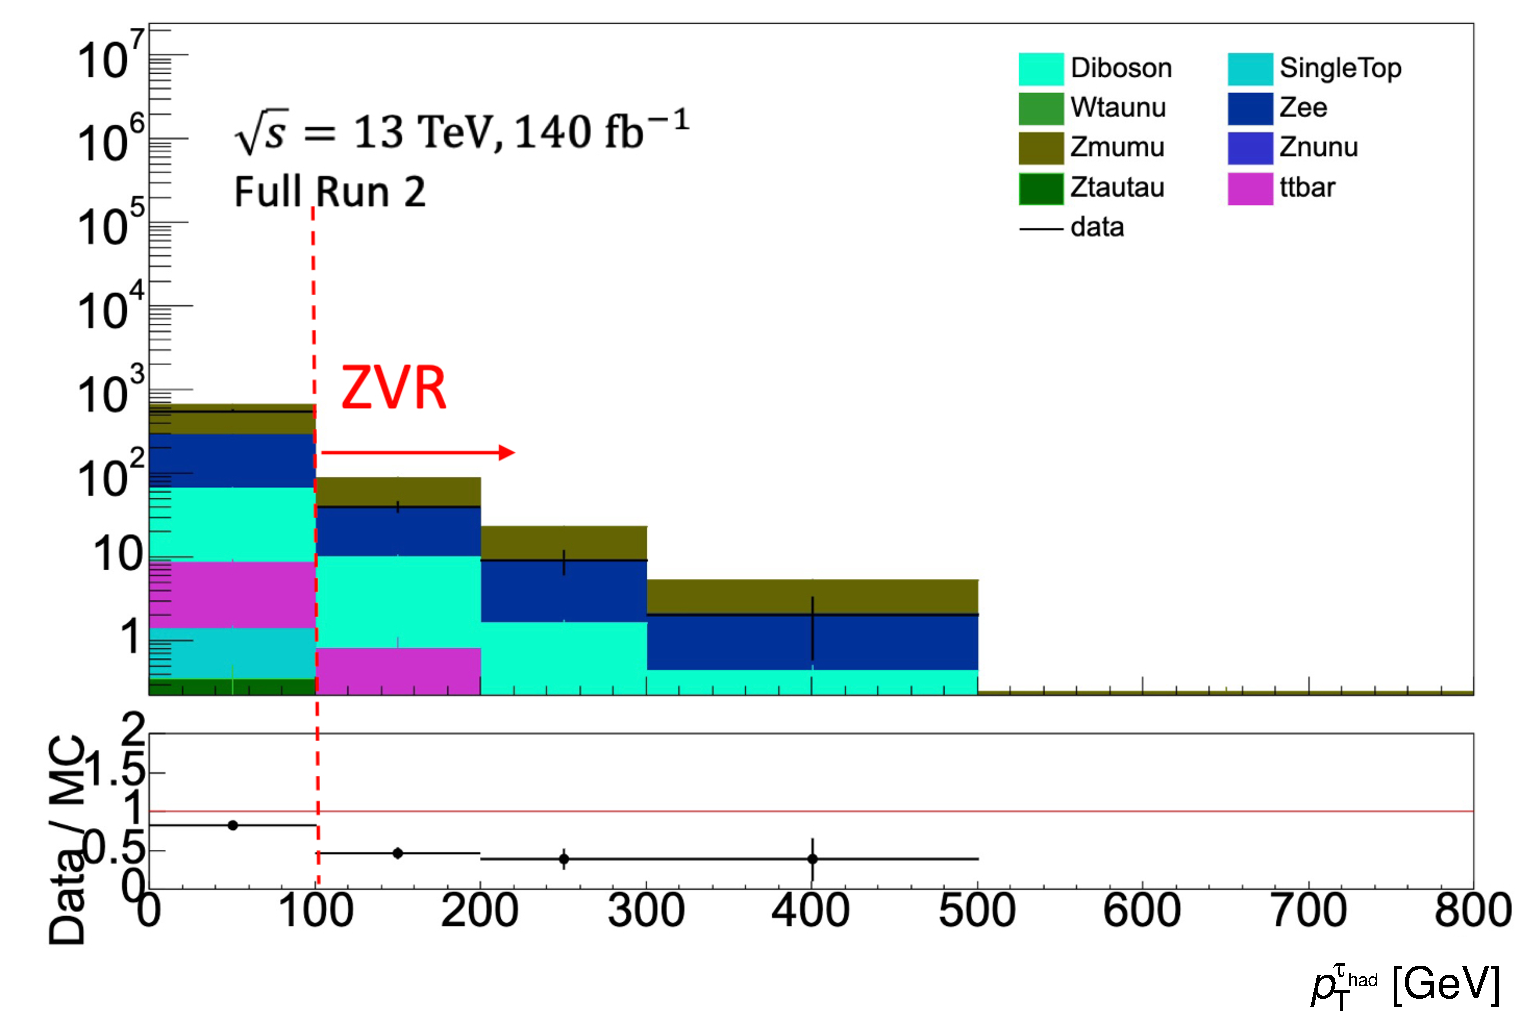
\includegraphics[width=0.80\linewidth]{Figs/CH8/fake_tau_appendix/ZVR_pTtau.pdf}
    \caption[Tau momentum distribution in the ZVR]{$N-1$ kinematic plot of $\pT^{\hadtau}$ in the ZVR. The mismodelling of fake $\hadtau$ in the tail region is observed.}
    \label{fig:ch8_zvr_pt}
\end{figure}

\begin{figure}[htpb]
    \centering
    \begin{subfigure}{0.49\linewidth}
        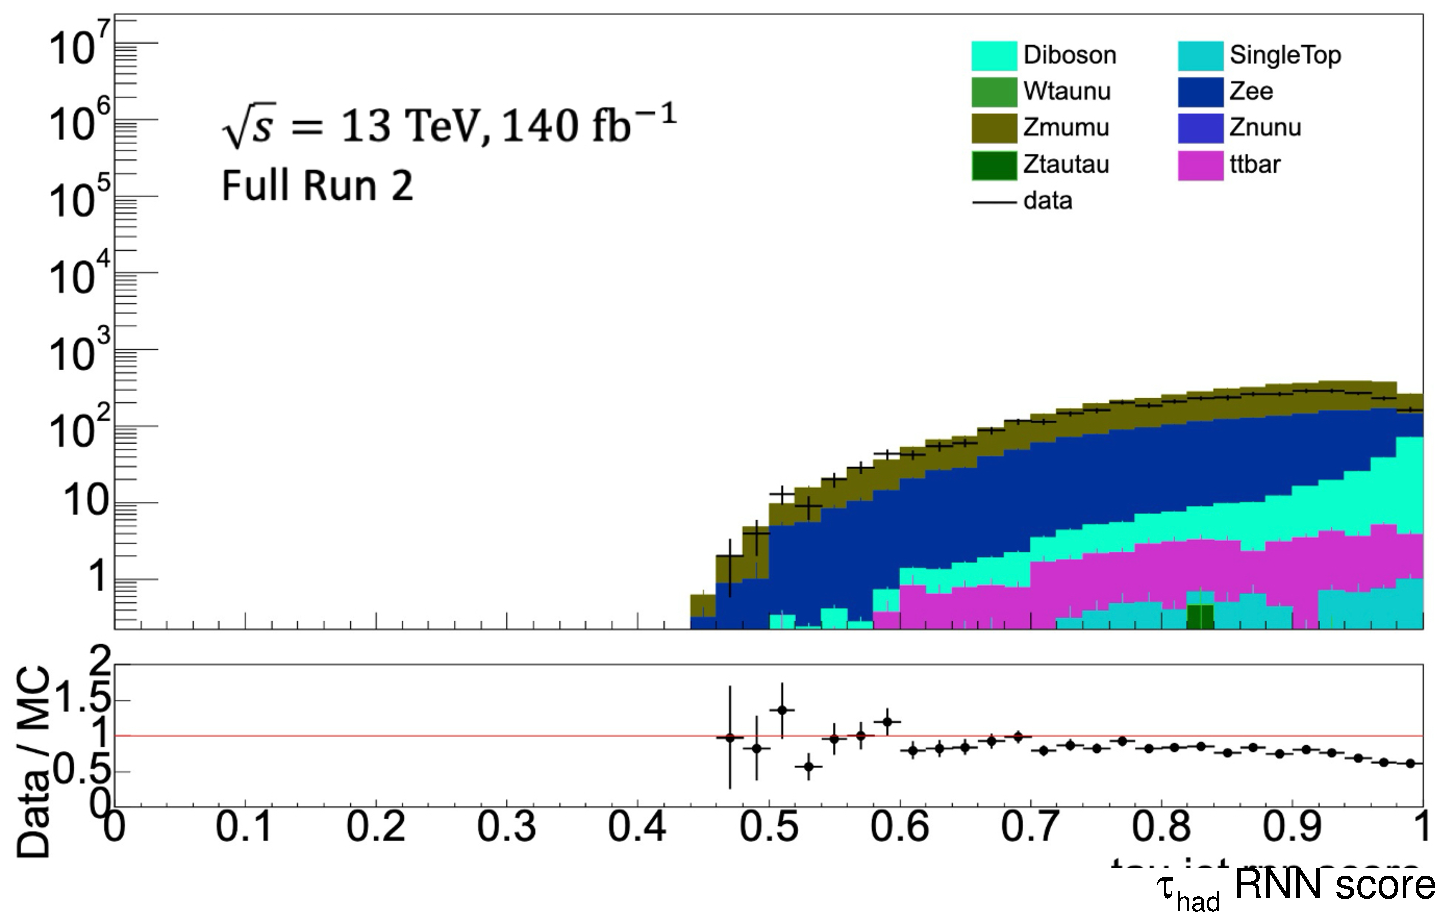
\includegraphics[width=\linewidth]{Figs/CH8/fake_tau_appendix/ZVR_1tau20GeV_score.pdf}
        \caption[]{$\pT^{\hadtau}>20~\GeV$}
    \end{subfigure}\hfill
    \begin{subfigure}{0.49\linewidth}
        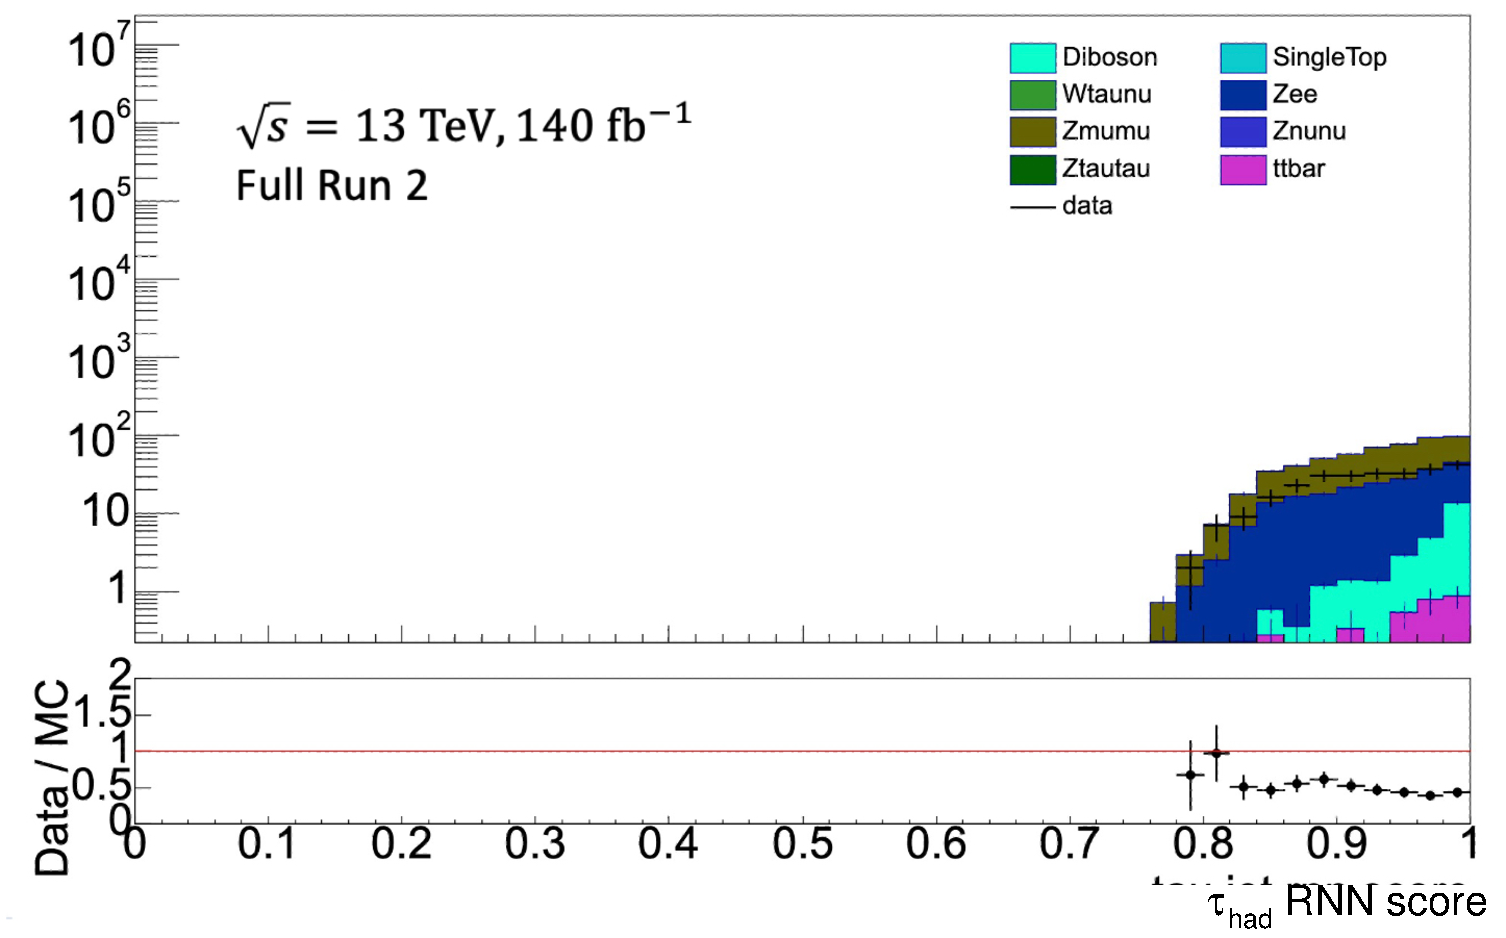
\includegraphics[width=\linewidth]{Figs/CH8/fake_tau_appendix/ZVR_1tau100GeV_score.pdf}
        \caption[]{$\pT^{\hadtau}>100~\GeV$}
    \end{subfigure}
    \caption[Tau-identification RNN distributions in the ZVR]{$\hadtau$-id RNN score in the regions of $\pT^{\hadtau}>20~\GeV$ (left) and $\pT^{\hadtau}>100~\GeV$ (right). Both figures use a loose $\hadtau$-id selection and a lower $\mT$ selection to observe the difference between high RNN score and low RNN score regions.}
    \label{fig:ch8_zvr_rnn}
\end{figure}

